\documentclass{standalone}
\usepackage{tikz}
\usepackage{ctex,siunitx}
\setCJKmainfont{Noto Serif CJK SC}
\usepackage{tkz-euclide}
\usepackage{amsmath}
\usetikzlibrary{patterns, calc}
\usetikzlibrary {decorations.pathmorphing, decorations.pathreplacing, decorations.shapes,}

\begin{document}
\small
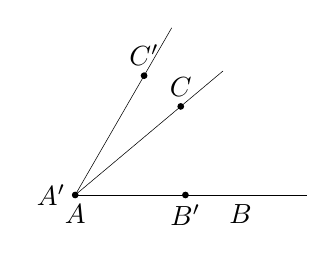
\begin{tikzpicture}[>=stealth,scale=0.7]
  \tkzSetUpPoint[fill=black]
  % \useasboundingbox(-1,-0.75)rectangle(3.7,1.4);
  \tkzDefPoints{0/0/A, 2/0/B', 3/0/B}
  \tkzDefPoint(40:2.5){C}
  \tkzDefPoint(60:2.5){C'}
  \tkzLabelPoints[below](A,B',B)
  \tkzLabelPoints[above](C,C')
  \tkzDrawLines[add=0 and .4 ](A,B A,C' A,C)
  \tkzDrawPoints(A,B',C',C)
  \node at (0,0)[left]{$A'$};
\end{tikzpicture}
\end{document}